\section{Index calculus over prime fields}
\label{sec:indexcalc}

Index calculus is the algorithm whose exponent is supposed to beat
one half. In $(\ZZ/p\ZZ)^*$ it does, near $56$~bits on this library.
On $E(\FF_p)$ and $E(\FF_{p^3})$ it does not, at any size that fits.
A genus-3/4 Jacobian is the positive control that shows the unit can
register a crossover when one exists.

\subsection{\texorpdfstring{Linear sieve in $(\ZZ/p\ZZ)^*$}{Linear sieve in (Z/pZ)*}}
\label{sec:ic-mult}

The library implements the Coppersmith--Odlyzko--Schroeppel linear
sieve~\cite{cos1986}. With $H=\lceil\sqrt{p}\rceil$ and $J=H^2-p$,
\[
  (H+c_1)(H+c_2) \;=\; J+(c_1+c_2)H+c_1c_2 \pmod{p},
\]
and the right-hand side is $O(C\sqrt{p})$ for $|c_i|\le C$, so it is
$B$-smooth far more often than a random residue. Unknowns are the logs
of the primes up to $B$ and of the $2C+1$ numbers $H+c$. Heuristic
complexity $L_p[1/2,1]$. Random-exponent collection ($L_p[1/2,2]$) is
kept as an independent check of the linear
algebra.\art{src/indexcalc.c}\art{docs/ALGORITHMS.md, ``Index calculus''}

Linear algebra is modulo $p-1=\prod q^e$. For $q\le 2^{24}$ the
factor-base logs are computed directly with Pohlig--Hellman in the
small subgroups. For each larger $q$ the relation matrix is solved
modulo $q$: structured Gaussian elimination, then Lanczos on $A^TDA$
with a random diagonal $D$ (LaMacchia--Odlyzko~\cite{lamacchia1990}),
Hensel-lifted for $e>1$. Every factor-base logarithm is verified
($\zeta^{\log}=q\bmod p$) before it is used. Individual logarithms
are randomised smoothness trials of $h\zeta^e$; at these sizes a few
hundred trial divisions suffice, so there is no descent stage.

Table~\ref{tab:ic-zp} is a re-run of \texttt{ca\_bench ic --threads 4}
on this machine, extended from the published $32$--$56$-bit table
through $60$ and $62$~bits. The $32$--$56$ columns match the published
factor-base and unknown counts; wall-clock differs because the host
differs. The $60$ and $62$-bit rows did not appear in the published
table and are marked as this extension.\art{paper/ic-rerun.txt}\art{docs/BENCHMARKS.md, Index calculus in (Z/pZ)*}

\begin{table}[t]
\centering
\small
\caption{Linear sieve in $(\ZZ/p\ZZ)^*$, safe primes $p=2q+1$, 4
  threads, this machine. ``rho ops'' is $1.3\sqrt{q}$. Rows $60$ and
  $62$ are the extension.}
\label{tab:ic-zp}
\begin{tabular}{@{}rrrrrrrr@{}}
\toprule
bits & fb & unk. & rels & sieve s & LA s & pre s & rho ops \\
\midrule
32 & 53 & 354 & 1\,290 & 0.002 & 0.013 & 0.015 & $4.3\cdot 10^{4}$ \\
40 & 125 & 926 & 1\,919 & 0.001 & 0.043 & 0.045 & $6.8\cdot 10^{5}$ \\
48 & 303 & 2\,504 & 3\,657 & 0.003 & 0.170 & 0.173 & $1.1\cdot 10^{7}$ \\
56 & 669 & 6\,270 & 7\,794 & 0.013 & 0.793 & 0.806 & $1.7\cdot 10^{8}$ \\
60$^*$ & 1\,007 & 10\,008 & 11\,396 & 0.014 & 1.614 & 1.629 & $7.0\cdot 10^{8}$ \\
62$^*$ & 1\,284 & 12\,785 & 14\,675 & 0.014 & 2.697 & 2.712 & $1.4\cdot 10^{9}$ \\
\bottomrule
\end{tabular}\\[0.3em]
{\footnotesize $^*$ extension, this machine; not in the published table.}
\end{table}

The sieve is essentially free; the cost is Lanczos, which grows as
$(\text{unknowns})^2$. At the published $Z_p^*$ rate of $169.4$~Mops/s,
rho at $56$~bits is about $1.0$~s of multiply-equivalents against
$0.81$~s of index-calculus precomputation on this host, confirming the
published crossover near $56$~bits. At $60$ and $62$~bits the same
conversion gives about $4.1$~s and $8.3$~s of rho against $1.63$~s and
$2.71$~s of sieve-plus-Lanczos: the gap widens, as $L_p[1/2]$ against
$N^{1/2}$ says it should. Individual logarithms remain negligible
($147$--$1{,}310$ trial divisions).

This is an $L_p[1/2,1]$ implementation. The state of the art above
roughly $100$~bits is the number field sieve ($L_p[1/3]$); NFS is out
of scope for a 64-bit toolkit.

\subsection{Elliptic curves: the negative, phase by phase}
\label{sec:ic-elliptic}

For elliptic curves over prime fields no index calculus is known that
beats rho at any cryptographic size~\cite{semaev2004,gaudry2009,diem2011}.
The sibling's boundary ledger puts three regimes --- a generic
prime-field curve, a random binary curve, and a Koblitz curve --- on
the same axis, every phase charged, every logarithm
verified.\art{crypto:research/notes/index-calculus/RESEARCH_IC_BOUNDARY_LEDGER.md}

Headline cells, full pipeline:

\begin{center}
\small
\begin{tabular}{@{}llrrr@{}}
\toprule
regime & best variant & $S$ & vs rho & vs floor \\
\midrule
prime, $23.4$-bit subgroup & MITM $m=3$ & $56.8$ & $14.5\times$ & $64.1\times$ \\
random binary, $24.4$-bit & MITM $m=3$ & $206$ & $89\times$ & $232\times$ \\
Koblitz, $39$-bit subgroup & orbit-column MITM & $58.8$ & $300\times$ & $425\times$ \\
\bottomrule
\end{tabular}
\end{center}

Matched rho on those instances: $S=3.93$ (prime), $S=2.31$ (binary),
signed-Frobenius $S=0.20$ (Koblitz). Fitted full-pipeline exponents:
prime MITM $m=3$ at $0.60$; binary MITM $m=3$ at $0.62$; Koblitz
signed-orbit MITM at $0.54$ overall, or $0.51$ on cofactor-${}\le 4$
rungs. All are above one half. No cell is below matched rho.

Oracle rounds that price only the decomposition of one residual are
stage diagnostics. They do not enter the $S$ column and are not
reported as speedups.

\subsection{\texorpdfstring{$E(\FF_{p^3})$ residual walks}{E(F_p^3) residual walks}}
\label{sec:ic-cubic}

The residual-walk note is the worked negative
(Section~\ref{sec:method-residual}). The prime-field route loses
because it has no proper additive subspace; the $S_3$ oracle pays per
base element. On $E(\FF_{p^3})$ a factor base that is an
$\FF_p$-subspace lets a residual be a walk, and the counting floor of
§9.6 applies.

A MITM triple oracle at $p=271$ to $2083$ ($n=2^{24.2}$ to $2^{33.1}$)
measures $S=1{,}224\to 3{,}805$, i.e.\ $1{,}057\times\to 2{,}240\times$
rho, fitted total exponent $0.69$ against a prediction of $2/3$.
Building a base-independent $S_4$ solve left an initial $C_3$ of
$4.7$--$4.9$ million $\FF_p$-multiplications per residual; the
relation-only crossover extrapolated to $2^{111}$. Engineering in
§§11.5--11.6 reduced $C_3$ to $879{,}000$, a $5.5\times$ improvement,
and the relation-only crossover became $2^{96}$. That $2^{96}$ is a
stage diagnostic.

Section~11.7 restores full accounting. Sequential Wiedemann over
$\ZZ/n\ZZ$, multiplications modulo $n\approx p^3$ charged as $9$
$\FF_p$ multiplications, every run correct
(Table~\ref{tab:gaudry-la}):\art{crypto:research/notes/index-calculus/RESEARCH_RESIDUAL_WALKS.md, §11.7}

\begin{table}[t]
\centering
\small
\caption{$E(\FF_{p^3})$ residual walks, full pipeline. $S$ includes
  relations, filtering and linear algebra. Every run recovered the
  planted logarithm.}
\label{tab:gaudry-la}
\begin{tabular}{@{}rrlrrr@{}}
\toprule
$p$ & $n$ & variant & $S$ & $S/$rho & LA share \\
\midrule
271 & $2^{24.2}$ & dense & 2\,696 & $2{,}328\times$ & $0.05\%$ \\
271 & $2^{24.2}$ & Wiedemann & 2\,830 & $2{,}443\times$ & $0.19\%$ \\
271 & $2^{24.2}$ & + large primes & 4\,634 & $4{,}000\times$ & $0.02\%$ \\
523 & $2^{27.1}$ & dense & 1\,989 & $1{,}680\times$ & $0.10\%$ \\
1\,039 & $2^{30.1}$ & dense & 1\,236 & $903\times$ & $0.31\%$ \\
2\,083 & $2^{33.1}$ & dense & 898 & $528\times$ & $1.22\%$ \\
2\,083 & $2^{33.1}$ & Wiedemann & 974 & $574\times$ & $1.61\%$ \\
2\,083 & $2^{33.1}$ & + large primes & 3\,378 & $1{,}989\times$ & $0.03\%$ \\
\bottomrule
\end{tabular}
\end{table}

Fitted exponents over the four sizes: dense total $n^{0.32}$,
Wiedemann linear algebra $n^{0.68}$ ($N^{2.00}$ in the number of
unknowns), double large primes total $n^{0.44}$ near $4/9$. Relations
cost $n^{1/3}$ and the linear algebra $n^{0.68}$ at best, so $S$ falls
as $n^{-1/6}$ while the linear-algebra term rises as $n^{+0.18}$.
Extrapolating the two measured terms, $S$ bottoms out at $\approx 265$
around $n\approx 2^{50}$ --- still $\approx 200\times$ rho --- and
rises after. Double large primes cost $1{,}989\times$ rho at $33$
bits; the extrapolated whole-method crossover is past $2^{230}$. Both
crossovers are extrapolations and are marked as such.

\subsection{Joux--Vitse pair-only}

Decompositions into $k-1$ points~\cite{jouxvitse2013} cut the
per-residual Groebner cost dramatically and grow the residual count.
Table~\ref{tab:paironly} is §11.9 of the residual-walk
note.\art{crypto:research/notes/index-calculus/RESEARCH_RESIDUAL_WALKS.md, §11.9}

\begin{table}[t]
\centering
\small
\caption{Joux--Vitse pair-only versus the $S_4$ hybrid, full
  pipeline. At $33$ bits the per-residual constant has improved about
  $580\times$ while residual growth wins: relabelling.}
\label{tab:paironly}
\begin{tabular}{@{}rrrrr@{}}
\toprule
$p$ & $n$ & $S$ & $S/$rho & residuals \\
\midrule
271 & $2^{24.2}$ & 427 & $534\times$ & 1\,513 \\
523 & $2^{27.1}$ & 1\,331 & $951\times$ & 1\,557 \\
1\,039 & $2^{30.1}$ & 1\,655 & $1{,}273\times$ & 1\,810 \\
2\,083 & $2^{33.1}$ & 1\,659 & $1{,}037\times$ & 1\,857 \\
\bottomrule
\end{tabular}
\end{table}

Residuals fit $n^{0.67}$, total $n^{0.72}$, so $S$ grows as
$n^{+0.22}$. Pair-only is the best local cell below roughly
$n=2^{28.5}$; at $33$ bits it is relabelling. Rho still costs
$S\approx 1.3$ and the best row in the table is $427$.

\subsection{Genus 3/4 Jacobian, the positive control}
\label{sec:ic-hyper}

Adleman--DeMarrais--Huang / Enge index calculus on a hyperelliptic
Jacobian of genus $g$ has predicted cost $O(g^2 q^{2-2/g+\varepsilon})$
against rho's $O(\sqrt{q^g})=O(q^{g/2})$. The ratio
$S_{\mathrm{IC}}/S_{\rho}$ should therefore fall as $N^{1/g-1/2}$:
flat at genus $2$, slope $-1/6$ at genus $3$, slope $-1/4$ at genus
$4$. Figure~\ref{fig:hyper} and Table~\ref{tab:hyper} are the sibling's
round-four/five measurements, every row a verified
$k$.\art{crypto:research/notes/index-calculus/RESEARCH_HYPERELLIPTIC_IC_RHO.md}

\begin{table}[t]
\centering
\small
\caption{Hyperelliptic index calculus versus distinguished-point rho.
  ``corr'' renormalises rho's walk to $\sqrt{\pi/2}$. Toy-sized,
  $p\le 251$.}
\label{tab:hyper}
\begin{tabular}{@{}rrrrrr@{}}
\toprule
$g$ & $p$ & $N$ & $S_{\mathrm{IC}}$ & $S_{\rho}$ & corr. ratio \\
\midrule
3 & 61 & 124\,459 & 1.51 & 2.30 & 0.73 \\
3 & 101 & 364\,747 & 1.12 & 1.90 & 0.64 \\
3 & 151 & 1\,180\,351 & 0.79 & 1.98 & 0.52 \\
3 & 211 & 4\,620\,611 & 0.53 & 1.96 & 0.38 \\
4 & 31 & 239\,753 & 1.77 & 1.90 & 0.95 \\
4 & 41 & 333\,041 & 1.41 & 1.86 & 0.80 \\
4 & 61 & 16\,790\,591 & 0.28 & 2.17 & \textbf{0.21} \\
\bottomrule
\end{tabular}
\end{table}

Fitted slopes against $\log_2 N$: genus $2$ at $-0.027$ ($R^2=0.24$,
no trend, prediction $0$); genus $3$ at $-0.154$ ($R^2=0.98$,
prediction $-1/6$); genus $4$ at $-0.275$ ($R^2=0.96$, prediction
$-1/4$). The law holds. Genus $3$ at $p=61$ and $p=101$ already sits
at $S_{\mathrm{IC}}/S_{\rho}=0.66$ and $0.61$ in the raw column; genus
$4$ at $p=61$, $N\approx 2^{24}$, reaches $0.21$ after the walk
renormalisation. That is the crossover this paper's unit was built to
see, and it appears on Jacobians, not on elliptic curves.

\begin{figure}[t]
\centering
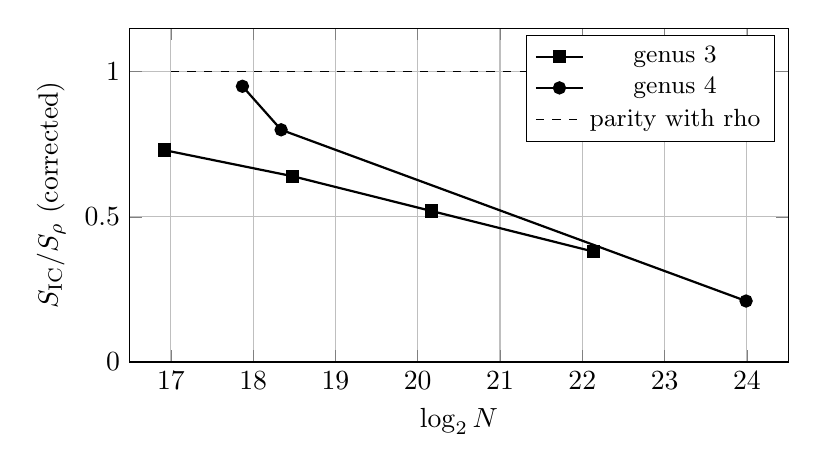
\begin{tikzpicture}
\begin{axis}[
  width=0.82\textwidth,
  height=0.48\textwidth,
  xlabel={$\log_2 N$},
  ylabel={$S_{\mathrm{IC}}/S_{\rho}$ (corrected)},
  xmin=16.5, xmax=24.5,
  ymin=0, ymax=1.15,
  grid=major,
  legend style={at={(0.98,0.98)},anchor=north east,font=\small},
]
\addplot[mark=square*,thick] coordinates {
  (16.92,0.73) (18.48,0.64) (20.17,0.52) (22.14,0.38)
};
\addlegendentry{genus 3}
\addplot[mark=*,thick] coordinates {
  (17.87,0.95) (18.34,0.80) (23.99,0.21)
};
\addlegendentry{genus 4}
\addplot[dashed,domain=17:24] {1};
\addlegendentry{parity with rho}
\end{axis}
\end{tikzpicture}
\caption{Hyperelliptic positive control. The ratio to distinguished-point
  rho falls at genus $3$ and genus $4$ with the predicted slopes.
  No measured end-to-end elliptic variant of Sections~\ref{sec:ic-elliptic}
  and~\ref{sec:ic-cubic} has crossed this line.}
\label{fig:hyper}
\end{figure}
